\chapter{Galois Theory}
Classical algebra was largely dedicated to finding the solutions to polynomials. The quadratic formula solved any equation of degree 2; the cubic formula any equation of degree 3; the quartic formula any equation of degree 4. However, a quintic formula eluded mathematicians for countless years, until Galois finally proved that such a task was impossible. In this penultimate chapter, we prove the Fundamental Theorem of Galois Theory and establish the insolvability of the quintic.

\section{Field Automorphisms}
Recall from \myref{section-automorphism-groups} that the set of automorphisms of a group forms a group, called the group of automorphisms. We note a similar result for that of field automorphisms.

\begin{proposition}
    The set of all automorphisms of a field $F$ is a group under function composition.
\end{proposition}
\begin{remark}
    We may reuse the notation used for the group of automorphisms of a group and denote the group of automorphisms of a field $F$ by $\Aut{F}$.
\end{remark}
\begin{proof}
    We prove the four group axioms.
    \begin{itemize}
        \item \textbf{Closure}: If $f, g \in \Aut{F}$, and $h = fg$, then $h: F \to F$ is a bijection. Furthermore $h$ is a homomorphism because for $x, y \in F$ we see
        \begin{align*}
            h(x+y) &= f(g(x + y))\\
            &= f(g(x) + g(y)) & (g \text{ is an isomorphism})\\
            &= f(g(x)) + f(g(y)) & (f \text{ is an isomorphism})\\
            &= h(x) + h(y)
        \end{align*}
        and
        \begin{align*}
            h(xy) &= f(g(xy))\\
            &= f(g(x)g(y)) & (g \text{ is an isomorphism})\\
            &= f(g(x))f(g(y)) & (f \text{ is an isomorphism})\\
            &= h(x)h(y).
        \end{align*}
        Therefore $h$ is a bijective homomorphism, meaning $h$ is an isomorphism. Because the domain and codomain of $h$ are both $F$, thus $h$ is an automorphism, meaning $h = fg \in \Aut{F}$.

        \item \textbf{Associativity}: Function composition is associative by \myref{axiom-function-composition-associative}.
        
        \item \textbf{Identity}: We have proved that the identity endomorphism is an automorphism (\myref{exercise-identity-homomorphism-is-an-isomorphism}) which means that $\id \in \Aut{F}$. By definition of $\id$ we know that $f\circ\id = f$ and $\id\circ f = f$ for any $f \in \Aut{F}$, meaning that $\id$ is indeed the identity of $\Aut{F}$.
        
        \item \textbf{Inverse}: Suppose $f \in \Aut{F}$, meaning $f$ is an automorphism. Then we know that $f^{-1}$ is an automorphism with
        \[
            f\circ f^{-1} = \id \text{ and } f^{-1} \circ f = \id
        \]
        which means that $f^{-1}$ is indeed the inverse of $f$.
    \end{itemize}
    Since the four group axioms are satisfied, therefore $\Aut{F}$ is a group under function composition.
\end{proof}

We are particularly interested in automorphisms of an extension field that fixes elements of the base field.
\begin{proposition}\label{prop-galois-group-is-group}
    Let $F$ be a field and $E/F$ a field extension. Then the set of all automorphisms of $E$ that fix $F$ elementwise is a group. In other words, the set of automorphisms $\phi: E \to E$ such that $\phi(a) = a$ for all $a \in F$ is a group.
\end{proposition}
\begin{proof}
    We show that this set is a subgroup of $\Aut{E}$. Note that $\id$ is an element of this subgroup since $\id(a) = a$ for all $a \in E$, including $a \in F$.

    Now suppose $\phi$ and $\psi$ be two automorphisms of $E$ such that $\phi(a) = a$ and $\psi(a) = a$ for all $a \in F$. Then we note that $\phi\psi^{-1}$ is an automorphism of $E$ with
    \begin{align*}
        \phi\psi^{-1}(a) &= \phi(\psi^{-1}(a))\\
        &= \phi(a) & (\text{since }\psi(a) = a \text{ thus } a = \psi^{-1}(a))\\
        &= a & (\text{since }\phi(a) = a)
    \end{align*}
    and so $\phi\psi^{-1}$ is an automorphism of $E$ that fixes $F$ elementwise.

    Therefore the result follows by the subgroup test.
\end{proof}

We have a special name for this group.
\begin{definition}
    Let $F$ be a field and $E/F$ a field extension. The group of all automorphisms of $E$ that fix $F$ elementwise is called the \textbf{Galois group of $E/F$}\index{Galois group} and is denoted $\Gal{E/F}$. That is,
    \[
        \Gal{E/F} = \left\{\phi \in \Aut{E} \vert \phi(a) = a \text{ for all } a \in F\right\}.
    \]
\end{definition}
\begin{remark}
    Let $F$ be a field. If $E$ is the splitting field of $f(x) \in F[x]$ over $F$, then the Galois group of $f(x)$ is $\Gal{E/F}$.
\end{remark}

\begin{example}
    One sees that $\phi: \C \to \C$ where $a+bi \mapsto a - bi$ is an automorphism. Since
    \[
        \phi(a) = \phi(a + 0i) = a - 0i = a
    \]
    for all $a \in \R$, therefore we see $\phi \in \Gal{\C/\R}$.
\end{example}

\begin{example}\label{example-galois-group-of-Q-sqrt3-sqrt5-over-Q}
    Consider the field $\Q \subset \Q(\sqrt5) \subset \Q(\sqrt3, \sqrt5)$. Then $\sigma: \Q(\sqrt3,\sqrt5) \to \Q(\sqrt3,\sqrt5)$ given by
    \[
        \sigma(a + b\sqrt3 + c\sqrt5 + d\sqrt{15}) = a - b\sqrt3 + c\sqrt5 - d\sqrt{15}
    \]
    is an automorphism. Also
    \[
        \sigma(a + b\sqrt{5}) = a+b\sqrt5
    \]
    so $\sigma$ fixes $\Q(\sqrt5)$. Similarly $\tau: \Q(\sqrt3,\sqrt5)\to\Q(\sqrt3,\sqrt5)$ given by
    \[
        \tau(a + b\sqrt3 + c\sqrt5 + d\sqrt{15}) = a + b\sqrt3 - c\sqrt5 - d\sqrt{15}
    \]
    is an automorphism that fixes $\Q(\sqrt3)$. The automorphism $\mu = \sigma\tau$ fixes $\Q(\sqrt{15})$. It will be clear soon that $S = \{\id, \sigma, \tau, \mu\}$ is $\Gal{\Q(\sqrt3,\sqrt5)/\Q}$.

    \begin{minipage}[c]{0.475\textwidth}
        \begin{table}[H]
            \centering
            \begin{tabular}{|l|l|l|l|l|}
                \hline
                & $\boldsymbol{\id}$ & $\boldsymbol{\sigma}$ & $\boldsymbol{\tau}$ & $\boldsymbol{\mu}$ \\ \hline
                $\boldsymbol{\id}$ & $\id$ & $\sigma$ & $\tau$ & $\mu$ \\ \hline
                $\boldsymbol{\sigma}$ & $\sigma$ & $\id$ & $\mu$ & $\tau$ \\ \hline
                $\boldsymbol{\tau}$ & $\tau$ & $\mu$ & $\id$ & $\sigma$ \\ \hline
                $\boldsymbol{\mu}$ & $\mu$ & $\tau$ & $\sigma$ & $\id$ \\ \hline
            \end{tabular}
        \end{table}
    \end{minipage}
    \begin{minipage}[c]{0.475\textwidth}
        \begin{table}[H]
            \centering
            \begin{tabular}{|l|l|l|l|l|}
                \hline
                & $\boldsymbol{(0, 0)}$ & $\boldsymbol{(0, 1)}$ & $\boldsymbol{(1, 0)}$ & $\boldsymbol{(1, 1)}$ \\ \hline
                $\boldsymbol{(0, 0)}$ & $(0, 0)$ & $(0, 1)$ & $(1, 0)$ & $(1, 1)$ \\ \hline
                $\boldsymbol{(0, 1)}$ & $(0, 1)$ & $(0, 0)$ & $(1, 1)$ & $(1, 0)$ \\ \hline
                $\boldsymbol{(1, 0)}$ & $(1, 0)$ & $(1, 1)$ & $(0, 0)$ & $(0, 1)$ \\ \hline
                $\boldsymbol{(1, 1)}$ & $(1, 1)$ & $(1, 0)$ & $(0, 1)$ & $(0, 0)$ \\ \hline
            \end{tabular}
        \end{table}
    \end{minipage}

    From the above tables, we see that $\Gal{\Q(\sqrt3,\sqrt5)/\Q} \cong \Z_2^2$. We also note that $[\Q(\sqrt3,\sqrt5):\Q] = 4$ by \myref{example-Q-sqrt3-sqrt5}. It is no coincidence that
    \[
        |\Gal{\Q(\sqrt3,\sqrt5)/\Q}| = [\Q(\sqrt3,\sqrt5):\Q] = 4
    \]
    as we will see later.
\end{example}

Why do we care about the Galois group? It turns out that an element of such a group (which is an automorphism) permutes the zeroes of a polynomial with coefficients in the base field.

\begin{proposition}\label{prop-galois-field-automorphism-permutes-zeroes-of-polynomial}
    Let $F$ be a field and $E/F$ a field extension. Let $f(x) \in F[x]$. Then any $\sigma \in \Gal{E/F}$ defines a permutation of the zeroes of $f(x)$ in $E$.
\end{proposition}
\begin{proof}[Proof (see {\cite[Proposition 23.5]{judson_beezer_2022}})]
    Let $f(x) = a_0 + a_1x + a_2x^2 + \cdots + a_nx^n$ and suppose $\alpha \in E$ is a zero of $f(x)$. Then for any $\sigma \in \Gal{E/F}$ we see
    \begin{align*}
        0 &= \sigma(0) & (\sigma \text{ fixes elements in }F)\\
        &= \sigma(f(\alpha)) & (\alpha \text{ is a zero of }f(x))\\
        &= \sigma(a_0 + a_1\alpha + a_2\alpha^2 + \cdots + a_n\alpha^n)\\
        &= a_0 + a_1\sigma(\alpha) + a_2\sigma(\alpha)^2 + \cdots + a_n(\sigma(\alpha))^n & (\sigma \text{ fixes elements in }F)
    \end{align*}
    which means that $\sigma(\alpha)$ is also a zero of $f(x)$.
\end{proof}

A partial converse of the above proposition exists for special kinds of elements, called conjugates.

\begin{definition}
    Let $F$ be a field and $E/F$ be a field extension. Two elements $\alpha,\beta \in E$ are \textbf{conjugate over $F$}\index{conjugate} if and only if they have the same minimal polynomial.
\end{definition}

\begin{example}
    In the field extension $\Q(\sqrt2)/\Q$, the elements $\sqrt2$ and $-\sqrt2$ are conjugates over $\Q$ since they are both zeroes of the minimal polynomial $x^2 - 2$.
\end{example}

\begin{example}
    In the field extension $\C/\R$, we see $i$ and $-i$ are conjugates over $\R$ since they are both zeroes of the minimal polynomial $x^2 + 1$.
\end{example}

\begin{proposition}
    Let $F$ be a field, $E/F$ be a field extension, and $\alpha,\beta \in E$ be conjugates over $F$. Then there exists an isomorphism $\sigma: F(\alpha) \to F(\beta)$ such that $\sigma(a) = a$ for all $a \in F$.
\end{proposition}
\begin{proof}
    Use \myref{lemma-isomorphism-extension} where, using the notation in that lemma, we set $F' = F$ and $\phi = \id$ and the result follows.
\end{proof}

We earlier found that $|\Gal{\Q(\sqrt3,\sqrt5)/\Q}| = [\Q(\sqrt3,\sqrt5):\Q] = 4$. We show that this is, in fact, not a coincidence.

\begin{theorem}\label{thrm-order-of-galois-group-is-degree-of-field-extension}
    Let $F$ be a field. Let $f(x) \in F[x]$ and suppose $E$ is the splitting field of $f(x)$ over $F$. If $f(x)$ only has simple zeroes, then
    \[
        |\Gal{E/F}| = [E:F],
    \]
    that is, the order of the Galois group of $E/F$ is equal to the degree of the field extension $E/F$.
\end{theorem}
\begin{proof}[Proof (cf. {\cite[Theorem 23.7]{judson_beezer_2022}})]
    We use strong induction on $[E:F]$.

    When $[E:F] = 1$, we have $E = F$ (\myref{prop-finite-extension-of-degree-1-means-extension-equals-base-field}). Therefore $\Gal{E/F}$ consists of only the identity automorphism and so $|\Gal{E/F}| = 1 = [E:F]$.

    Now assume that for any field $F'$, any $\mathfrak{f}(x) \in F'[x]$, and the splitting field $E'$ of $\mathfrak{f}(x)$ over $F'$ such that $[E':F'] \leq k$ for some positive integer $k$, that $|\Gal{E'/F'}| = [E':F']$. We show that the theorem holds for a field $F$, a polynomial $f(x) \in F[x]$, and the splitting field $E$ of $f(x)$ over $F$ such that $[E:F] = k+1$, i.e. we are to show $|\Gal{E/F}| = k + 1$.

    Let $f(x) = p(x)q(x)$, where $p(x), q(x) \in E[x]$ and $p(x)$ is irreducible of degree $d$. If $d = 1$, then $f(x)$ has a zero in $F$ and so $p(x) \in F[x]$. This thus means that $q(x) \in F[x]$ also, and thus $E = F$ which leads to $[E:F] = 1$. If instead $d > 1$, let $\alpha \in E$ be a zero of $p(x)$. Using \myref{lemma-isomorphism-extension} where we pick $F' = F$, $\phi = \id$, and $\beta$ to be a zero of $p(x)$ in $E$, we obtain an isomorphism $\phi: F(\alpha) \to F(\beta)$ where elements of $F$ are fixed under $\phi$ and where $\alpha$ is mapped to $\beta$, i.e. $\beta = \phi(\alpha)$. Since $f(x)$ only has simple zeroes, thus $p(x)$ has $d$ distinct zeroes in $E$, say $\beta_1, \beta_2, \dots, \beta_d$. By \myref{prop-galois-field-automorphism-permutes-zeroes-of-polynomial} we therefore see that there are exactly $d$ isomorphisms $\sigma: F(\alpha) \to F(\beta_i)$ that fix $F$, one for each zero $\beta_1, \beta_2, \dots, \beta_d$ of $p(x)$.

    Since $E$ is a splitting field of $f(x)$ over $F$, thus $E$ is also a splitting field of $f(x)$ over $F(\alpha)$. Similarly $E$ is a splitting field of $f(x)$ over $F(\beta)$. By Tower Law (\myref{thrm-tower-law}) one notes that
    \[
        k+1 = [E:F] = [E:F(\alpha)]\underbrace{[F(\alpha):F]}_{d}
    \]
    and so $[E:F(\alpha)] = \frac{k + 1}{d}$. By Induction Hypothesis, this means that $|\Gal{E:F(\alpha)} = \frac{k+1}{d}$. In other words, there are $\frac{k+1}{d}$ automorphisms $\psi: E \to E$ that fix $F(\alpha)$. But there are $d$ isomorphisms $\sigma: F(\alpha) \to F(\beta_i)$ that fix $F$. Therefore there must be $\frac{k+1}{d} \times d = k+1$ choices for an automorphism in $\Aut{E}$ that fixes $F$, i.e. $|\Gal{E/F}| = k+1$ as required.

    By mathematical induction the claim is proven.
\end{proof}

\begin{corollary}
    Let $F$ be a finite field with a finite extension $E$ such that $[E:F] = k$. Then $\Gal{E/F}$ is cyclic with order $k$.
\end{corollary}
\begin{proof}
    Let $p$ be the characteristic of $E$ and $F$, and assume that the orders of $E$ and $F$ are $p^m$ and $p^n$ respectively. Then by \myref{thrm-subfields-of-finite-field} we know that $m = nk$. Also by \myref{thrm-finite-field-is-unique} we may assume that $E$ is the splitting field of $x^{p^m} - x$ over a subfield of $E$ of order $p$. In particular this means that $E$ must be the splitting field of $x^{p^m} - x$ over $F$. Since $[E:F] = k$ thus $|\Gal{E/F}| = k$ by \myref{thrm-order-of-galois-group-is-degree-of-field-extension}.

    To prove that $\Gal{E/F}$ is cyclic we need to find a generator of $\Gal{E/F}$. In particular we need to find an isomorphism in $\Gal{E/F}$ of order $k$. Consider the map $\sigma: E \to E$ where $\phi(a) = a^{p^n}$ for any $a \in E$. We show that $\sigma \in \Aut{E}$.
    \begin{itemize}
        \item \textbf{Homomorphism}: Note that if $a, b \in E$ then
        \begin{align*}
            \sigma(a+b) &= (a+b)^{p^n}\\
            &= a^{p^n} + b^{p^n} & (\myref{prop-freshman-dream})\\
            &= \sigma(a) + \sigma(b)
        \end{align*}
        and
        \begin{align*}
            \sigma(ab) &= (ab)^{p^n}\\
            &= a^{p^n}b^{p^n}\\
            &= \sigma(a)\sigma(b)
        \end{align*}
        which means that $\sigma$ is a homomorphism.
        
        \item \textbf{Injective}: Since $\sigma$ is non-trivial it must be injective by \myref{thrm-homomorphism-from-field-is-injective-or-trivial}.
        
        \item \textbf{Surjective}: By \myref{problem-injection-from-finite-set-to-itself-is-bijection} we know that $\sigma$ is surjective.
    \end{itemize}
    Therefore $\sigma$ is an isomorphism from $E$ to $E$, i.e. $\sigma$ is an automorphism. So $\sigma \in \Aut{E}$.
    
    We also note that because $F$ is the splitting field of $x^{p^n}-x$ over the base field of order $p$, therefore every element of $F$ is a zero of $x^{p^n}-x$, in particular $a^{p^n} - a = 0$ which means $a = a^{p^n}$ for any $a \in F$. Hence $\sigma(a) = a$ for all $a \in F$, which shows that $\sigma \in \Gal{E/F}$.

    Finally we show that the order of $\sigma$ in $\Gal{E/F}$ is $k$. Recall that since $E$ is the splitting field of $x^{p^m} - x$ over the base field of order $p$, therefore every element of $E$ is a zero of $x^{p^m} - x$ which results in $a^{p^m} = a$ for all $a \in E$. Thus one sees that
    \begin{align*}
        (\sigma^k)(a) &= a^{p^{nk}}\\
        &= a^{p^m}\\
        &= a
    \end{align*}
    for all $a \in E$, meaning that $\sigma^k$ is the identity of $\Gal{E/F}$. We also see that $\sigma^r$ cannot be the identity for $1 \leq r < k$ since otherwise $x^{p^{nr}} - x$ would have $p^m$ roots while the polynomial itself has a degree of $p^{nr}$, which is less than $p^m$, contradicting \myref{thrm-polynomial-of-degree-n-has-at-most-n-zeroes}. Therefore $|\sigma| = k$ in $\Gal{E/F}$, showing that $\Gal{E/F}$ is cyclic with order $k$.
\end{proof}

\begin{example}
    Remember when we claimed that $\Gal{\Q(\sqrt3,\sqrt5)/\Q} \cong \Z_2^2$ in \myref{example-galois-group-of-Q-sqrt3-sqrt5-over-Q}? Certainly $H = \{\id, \sigma, \tau, \mu\}$ is a subgroup of $\Gal{\Q(\sqrt3,\sqrt5)/\Q}$. However one sees that $|H| = 4$ and
    \[
        |\Gal{\Q(\sqrt3,\sqrt5)/\Q}| = [\Q(\sqrt3,\sqrt5):\Q] = 4
    \]
    by \myref{thrm-order-of-galois-group-is-degree-of-field-extension}. Therefore $H = \Gal{\Q(\sqrt3,\sqrt5)/\Q}$.
\end{example}

\begin{exercise}
    Consider the field extension $\C/\R$.
    \begin{partquestions}{\roman*}
        \item Find the order of $\Gal{\C/\R}$.
        \item Find the element(s) of $\Gal{\C/\R}$.
    \end{partquestions}
\end{exercise}

\section{Separable Extensions}
For many results, we are interested in polynomials with only simple zeroes within its splitting field over the base field. These polynomials are called separable polynomials.

\begin{definition}
    Let $F$ be a field and $f(x) \in F[x]$. Let $E$ be the splitting field of $f(x)$ over $F$. Then $f(x)$ is called \textbf{separable}\index{polynomial!separable} if and only if it has only simple zeroes in $E$. In other words, over $E$,
    \[
        f(x) = a(x-\alpha_1)(x-\alpha_2)\cdots(x-\alpha_n)
    \]
    where each $\alpha_i$ is distinct.
\end{definition}

Recall that \myref{thrm-criterion-for-multiple-zeroes} tells us that a polynomial $f(x)$ has multiple zeroes if and only if $\deg \gcd(f(x), f'(x)) > 0$. Therefore a polynomial $f(x)$ has only simple zeroes if and only if $\gcd(f(x), f'(x)) = k$, a constant in $F$.

Recall also from \myref{thrm-zeroes-of-an-irreducible} that an irreducible polynomial in $F[x]$ is separable if
\begin{itemize}
    \item $\Char{F} = 0$; or
    \item $\Char{F} = p$, a prime, and $f(x) \neq g(x^p)$ for some $g(x) \in F[x]$.
\end{itemize}

\begin{definition}
    Let $F$ be a field. An extension $E$ is a \textbf{separable extension}\index{extension!separable} of $F$ if and only if every element of $E$ is a zero of a separable polynomial in $F[x]$.
\end{definition}

Separable extensions are nice in the way that they can be determined solely by one primitive element. Before we can prove this fact, we note one lemma.

\begin{lemma}\label{lemma-primitive-element}
    Let $F$ be an infinite field and $E$ a finite separable extension of $F$. If $E = F(a, b)$ then there exists a $c \in E$ such that $E = F(c)$.
\end{lemma}
\begin{proof}[Proof (see {\cite[Theorem 21.6]{gallian_2016}} and {\cite[Theorem 23.13]{judson_beezer_2022}})]
    Let $p(x)$ and $q(x)$ be the minimal polynomials over $F$ for $a$ and $b$ respectively. Let $K/F$ be a field extension where $a_1, a_2, \dots, a_m$ and $b_1, b_2, \dots, b_n$ are the zeroes of $p(x)$ and $q(x)$ in $K$, and where $a = a_1$ and $b = b_1$. Choose a $d \in F$ such that
    \[
        d \neq (a_i-a)(b-b_j)^{-1}
    \]
    for all $i \in \{1, 2, 3, \dots, m\}$ and $j \in \{2, 3, \dots, n\}$. In other words we have $a_i \neq a + d(b-b_j)$ for all $i \in \{1, 2, 3, \dots, m\}$ and $j \in \{2, 3, \dots, n\}$.

    Now we show that $c = a + db$ has the property that $F(a, b) = F(c)$. Clearly $F(c) \subseteq F(a, b)$; we just need to show $F(a, b) \subseteq F(c)$. We note that $a = c - db$, so we just need to prove that $b \in F(c)$ and this would automatically imply that $a \in F(c)$ and therefore $F(a,b) \subseteq F(c)$.

    Consider the polynomial $r(x) = p(c - dx)$, i.e. $r(x)$ is obtained by substituting $c - dx$ for $x$ in $p(x)$. One then sees that $q(b) = 0$ (by definition of the minimal polynomial of $b$ over $F$) and $r(b) = p(c - db) = p(a) = 0$, so both $q(x)$ and $r(x)$ are divisible by the minimal polynomial for $b$ over $F(c)$ by \myref{corollary-minimal-polynomial-divides-polynomial-with-same-root}. Let $s(x) \in F(c)[x]$ be the minimal polynomial of $b$ over $F(c)$. Since $s(x)$ is a common divisor of both $q(x)$ and $r(x)$, thus the only possible zeroes of $s(x)$ in $K$ are the zeroes of $q(x)$ that are also zeroes of $r(x)$. But note
    \begin{align*}
        r(b_j) &= p(c-db_j)\\
        &= p((a+db) - db_j)\\
        &= p(a+d(b-b_j))
    \end{align*}
    and $a_i \neq a+d(b-b_j)$ for all $i \in \{1, 2, 3, \dots, m\}$ and $j \in \{2, 3, \dots, n\}$. Therefore the only possible zero of $s(x)$ in $K$ is $b_1 = b$; consequently $s(x) = (x-b)^u$ for some positive integer $u$. However $s(x)$ is irreducible (by definition of a minimal polynomial), and because $F$ has characteristic 0, therefore $s(x)$ has no multiple zeroes (\myref{thrm-zeroes-of-an-irreducible}), meaning $u = 1$ and therefore $s(x) = x-b$. The only zero of $s(x)$ is clearly $b$, and by definition of a minimal polynomial, we must have $b \in F(c)$, proving $F(a, b) \subseteq F(c)$.

    So we have $F(c) \subseteq F(a, b)$ and $F(a, b) \subseteq F(c)$, proving that $F(a, b) = F(c)$.
\end{proof}

\begin{theorem}[Primitive Element Theorem]\index{Primitive Element Theorem}\label{thrm-primitive-element}
    Every separable field extension of finite degree is simple.
\end{theorem}
\begin{proof}
    Let $E$ be a finite separable extension of a field $F$. We show that there exists an $\alpha \in E$ such that $E = F(\alpha)$.

    For the case when $F$ is finite, we know that $E$ is also finite (\myref{thrm-subfields-of-finite-field}) and so $E^\ast$ is cyclic (\myref{thrm-structure-of-finite-field}). Let $\alpha$ be a generator of $E^\ast$. Then one sees that $E = F(\alpha)$.

    For the case when $F$ is infinite, suppose $[E:F] = n$, which means that we may write $E = F(a_1, a_2, \dots, a_n)$ where each $a_i$ is in $E$. We induct on $n$. We choose $n > 1$ since the case of $n = 1$ would lead to $E = F$ (\myref{prop-finite-extension-of-degree-1-means-extension-equals-base-field}).

    When $n = 2$, then $E = F(a_1, a_2)$. \myref{lemma-primitive-element} immediately gives us a $\alpha \in E$ such that $E = F(\alpha)$.

    Assume for some positive integer $k$ that if $E = F(a_1, a_2, \dots, a_k)$ then there exists an $\alpha \in E$ such that $E = F(\alpha)$. We show that this holds for the case of $k + 1$.

    If $[E:F] = k + 1$ this means that $E = F(a_1, a_2, \dots, a_k, a_{k+1})$. Thus
    \begin{align*}
        F(a_1, a_2, \dots, a_k, a_{k+1}) &= F(a_1, a_2, \dots, a_k)(a_{k+1}) & (\myref{prop-field-generated-by-S-inductive-definition})\\
        &= F(\alpha_1)(a_{k+1}) \text{ for some } \alpha_1 \in E & (\text{Induction Hypothesis})\\
        &= F(\alpha_1, a_{k+1}) & (\myref{prop-field-generated-by-S-inductive-definition})\\
        &= F(\alpha) \text{ for some } \alpha \in E & (\myref{lemma-primitive-element})
    \end{align*}
    which proves the case for $k + 1$.
\end{proof}

\section{Fixed Fields}
\begin{definition}
    Let $F$ be a field and $E/F$ be a field extension. Let $H$ be a subgroup of $\Gal{E/F}$. Then the \textbf{fixed field}\index{fixed field} of $H$ is
    \[
        \Fix{E}{H} = \{x \in E \vert \phi(x) = x \text{ for all } \phi \in H\}.
    \]
\end{definition}
\begin{remark}
    Other authors may choose to denote the fixed field of $H$ by $E_H$ (e.g. \cite[p.~531]{gallian_2016} and \cite[p.~298]{judson_beezer_2022}) or by $E^H$ (e.g. \cite[p.~486]{artin_2011}).
\end{remark}

\begin{proposition}\label{prop-fixed-field-is-subfield}
    Let $F$ be a field, $E/F$ a field extension, and $H$ be a subgroup of $\Gal{E/F}$. Then $\Fix{E}{H}$ is a subfield of $E$.
\end{proposition}
\begin{proof}
    See \myref{exercise-fixed-field-is-subfield} (later).
\end{proof}

\begin{example}
    Consider the field $\Q(\sqrt3,\sqrt5)$, and the automorphism $\sigma$ on that field such that $\sqrt3 \mapsto -\sqrt3$. Then the fixed field of $\langle\sigma\rangle$ is $\Q(\sqrt5)$, i.e. $\Fix{E}{\langle\sigma\rangle} = \Q(\sqrt5)$.
\end{example}

\begin{exercise}\label{exercise-fixed-field-is-subfield}
    Prove \myref{prop-fixed-field-is-subfield}.
\end{exercise}

\begin{proposition}\label{prop-fixed-field-of-Gal-E/F-is-F}
    Let $F$ be a field. Let $E$ be the splitting field of a separable polynomial $f(x) \in F[x]$ over $F$. Then
    \[
        \Fix{E}{\Gal{E/F}} = F.
    \]
\end{proposition}
\begin{proof}[Proof (cf. {\cite[Proposition 23.17]{judson_beezer_2022}})]
    For brevity let $G = \Gal{E/F}$.
    
    Note that $\Fix{E}{G} = \{a \in E \vert \phi(a) = a \text{ for all } \phi \in \Gal{E/F}\}$. But clearly every element of $F$ is fixed by any $\phi \in \Gal{E/F}$. Hence it is safe to say that $F \subseteq \Fix{E}{G}$. It is also clear that $\Fix{E}{G} \subseteq E$ since $\Fix{E}{G}$ is a subfield of $E$.

    Now since $F \subseteq \Fix{E}{G}$, any automorphism of $E$ that fixes $\Fix{E}{G}$ must also fix $F$. Thus $\Gal{E/\Fix{E}{G}} \subseteq \Gal{E/F}$. But by \myref{exercise-subgroup-of-Aut-E-is-subgroup-of-galois-group-of-fixed-field} (later) we see $\Gal{E/F} \leq \Gal{E/\Fix{E}{G}}$. Hence $\Gal{E/F} = \Gal{E/\Fix{E}{G}}$. Consequently, by \myref{thrm-order-of-galois-group-is-degree-of-field-extension} we see
    \[
        [E:F] = [E:\Fix{E}{G}].
    \]
    On the other hand, by Tower Law (\myref{thrm-tower-law}), one obtains
    \[
        [E:F] = [E:\Fix{E}{G}][\Fix{E}{G}:F].
    \]
    Therefore $[\Fix{E}{G}:F] = 1$ which yields $\Fix{E}{G} = F$ (\myref{prop-finite-extension-of-degree-1-means-extension-equals-base-field}), which is what was to be shown.
\end{proof}

\begin{exercise}\label{exercise-subgroup-of-Aut-E-is-subgroup-of-galois-group-of-fixed-field}
    Let $E$ be a field, $G$ be a subgroup of $\Aut{E}$, and $F = \Fix{E}{G}$. Show $G \leq \Gal{E/F}$.
\end{exercise}

\begin{theorem}\label{thrm-degree-of-element-under-fixed-field-action}
    Let $E$ be a field, $G$ be a finite subgroup of $\Aut{E}$, and $F = \Fix{E}{G}$. Define the group action of $G$ on $E$ by $\sigma \cdot x = \sigma(x)$ for all $x \in E$ and $\sigma \in G$. For some $\alpha_1 \in E$, let $\Orb{G}{\alpha_1} = \{\alpha_1, \alpha_2, \dots, \alpha_r\}$ where $r = |\Orb{G}{\alpha_1}|$. Then
    \begin{itemize}
        \item the minimal polynomial for $\alpha_1$ over $F$ is $(x-\alpha_1)(x-\alpha_2)\cdots(x-\alpha_r)$;
        \item $\alpha_1$ is algebraic over $F$ with degree equal to $r$; and
        \item the degree of $\alpha_1$ over $F$ divides $|G|$.
    \end{itemize}
\end{theorem}
\begin{proof}[Proof (see {\cite[Theorem 16.5.2]{artin_2011}})]
    We only prove the first two parts and leave the third for \myref{exercise-degree-of-element-under-fixed-field-action} (later).
    
    For the first part, say
    \[
        f(x) = (x-\alpha_1)(x-\alpha_2)\cdots(x-\alpha_r).
    \]
    We note that $G$ permutes the zeroes of the polynomial $f(x)$, so the coefficients of $f(x)$ remain unchanged. So every coefficient of $f(x)$ must belong in $\Fix{G}{E} = F$, and so $f(x) \in F[x]$.

    Now suppose $h(x) \in F[x]$ has a zero of $\alpha_1$. As $\Orb{G}{\alpha_1} = \{\alpha_1, \alpha_2, \dots, \alpha_r\}$, there exists a $\sigma \in G$ such that $\sigma(\alpha_1) = \alpha_i$ for some $i = 1, 2, \dots, r$. We note that $\alpha_i$ is a zero of $h(x)$ since, if we write $h(x) = a_0 + a_1x + \cdots + a_mx^m$, we see
    \begin{align*}
        0 &= \sigma(0)\\
        &= \sigma(f(\alpha_1))\\
        &= \sigma(a_0) + \sigma(a_1)\sigma(\alpha_1) + \cdots + \sigma(a_m)\sigma(\alpha_1^m)\\
        &= a_0 + a_1\sigma(\alpha_1) + \cdots + a_m\sigma(\alpha_1)^m\\
        &= a_0 + a_1\alpha_i + \cdots + a_m\alpha_i^m.
    \end{align*}
    Therefore $x - \alpha_i$ is a factor of $h(x)$ by Factor Theorem (\myref{corollary-factor-theorem}). Since this is true for every $i = 1, 2, \dots, r$, therefore $(x-\alpha_1)(x-\alpha_2)\cdots(x-\alpha_r) = f(x)$ is a factor of $h(x)$. So $f(x)$ divides every polynomial with a zero of $\alpha_1$, including the minimal polynomial of $\alpha_1$. But the minimal polynomial of $\alpha_1$ divides every polynomial with a zero of $\alpha_1$ (\myref{corollary-minimal-polynomial-divides-polynomial-with-same-root}), which means that $f(x)$ is the minimal polynomial of $\alpha_1$.

    Now clearly since $\alpha_1$ has a minimal polynomial of $f(x) \in F[x]$, it is thus algebraic. Furthermore the extension $F(\alpha)$ has degree $r$. Therefore $\alpha$ has degree $r$.
\end{proof}

\begin{exercise}
    Prove that the group action defined in \myref{thrm-degree-of-element-under-fixed-field-action} is indeed a group action.
\end{exercise}

\begin{exercise}\label{exercise-degree-of-element-under-fixed-field-action}
    Prove that the degree of $\alpha_1$ over $F$ in \myref{thrm-degree-of-element-under-fixed-field-action} divides $|G|$.
\end{exercise}

We end this section with the Fixed Field Theorem.

\begin{theorem}[Fixed Field Theorem]\index{Fixed Field Theorem}\label{thrm-fixed-field}
    Let $F$ be a field and $E/F$ be a field extension such that $F = \Fix{E}{G}$ for some finite subgroup $G$ of $\Aut{E}$. Then $|G| = [E:F]$.
\end{theorem}
\begin{proof}[Proof (see {\cite[Theorem 16.5.4]{artin_2011}})]
    For brevity let $n = |G|$. By \myref{thrm-degree-of-element-under-fixed-field-action} we know that the extension $E/F$ is algebraic since any element in $E$ is a zero of a polynomial in $F[x]$. In particular, the degree of any element $\alpha \in E$ divides $n$, meaning that the degree of an element in $E$ is at most $n$. Therefore the contrapositive of \myref{corollary-infinite-algebraic-extension-has-elements-of-arbitrarily-large-degree} tells us that $[E:F]$ is finite. Also, any element within $E$ is a zero of a separable polynomial in $F[x]$ by \myref{thrm-degree-of-element-under-fixed-field-action}. By the Primitive Element theorem (\myref{thrm-primitive-element}) we therefore can find a primitive element (say $\gamma$) of $E$, i.e. $E = F(\gamma)$.

    Now consider the group $G$ acting on $E$ by the group action $\sigma\cdot x = \sigma(x)$ for any $\sigma \in G$ and $x \in E$. We consider $\Stab{G}{\gamma}$. Note that because $\gamma \notin F = \Fix{E}{G}$, therefore the only element of $G$ that fixes $\gamma$ is $\id$, i.e. $\Stab{G}{\gamma} = \{\id\}$. By the Orbit-Stabilizer theorem (\myref{thrm-orbit-stabilizer}),
    \[
        n = |G| = |\Stab{G}{\gamma}||\Orb{G}{\gamma}|.
    \]
    Consequently $|\Orb{G}{\gamma}| = n$. Therefore \myref{exercise-degree-of-element-under-fixed-field-action} tells us that $\gamma$ has degree $n$ over $F$. Since $E = F(\gamma)$, one sees that $[E:F] = n$ too.
\end{proof}

\section{Galois Extensions}
We first define normal extensions.

\begin{definition}
    Let $F$ be a field and $E$ an algebraic extension of $F$. Then $E$ is called a \textbf{normal extension}\index{extension!normal} of $F$ if and only if every irreducible polynomial in $F[x]$ with \textit{at least one} zero in $E$ has \textit{all} of its zeroes in $E$. In other words, every irreducible polynomial in $F[x]$ with a zero in $E$ splits in $E$.
\end{definition}

Later we will see that normal extensions are, in some way, related to normal subgroups.

\begin{proposition}\label{prop-intermediate-field-of-normal-extension-is-normal-extension}
    Let $F$ be a field and $E$ be a normal extension of $F$. If $K$ is a field such that $F \subseteq K \subseteq E$, then $E$ is a normal extension of $K$.
\end{proposition}
\begin{proof}
    Let $f(x) \in K[x]$ be an irreducible polynomial, and let $\alpha \in E$ be a zero of $f(x)$. We can then find the minimal polynomial of $\alpha$ in $F[x]$, say $p(x) \in F[x]$. Since $E/F$ is a normal extension, thus $p(x)$ splits in $E$. Furthermore by \myref{corollary-minimal-polynomial-divides-polynomial-with-same-root}, if we view $p(x)$ as a polynomial in $K[x]$, then $p(x)$ divides $f(x)$. Now because $f(x)$ is irreducible over $K$, thus $f(x)$ has no zeroes in $K$; this means that $f(x)$ must split completely in $E$, showing that $E/K$ is a normal extension.
\end{proof}

\begin{definition}
    Let $F$ be a field. A normal separable field extension $E/F$ is called a \textbf{Galois extension}\index{extension!Galois} of $F$.
\end{definition}

\begin{proposition}\label{prop-intermediate-field-of-galois-extension-is-galois-extension}
    Let $F$ be a field and $E$ be a Galois extension of $F$. If $K$ is a field such that $F \subseteq K \subseteq E$, then $E$ is a Galois extension of $K$.
\end{proposition}
\begin{proof}
    See \myref{exercise-intermediate-field-of-galois-extension-is-galois-extension} (later).
\end{proof}

\begin{theorem}\label{thrm-equivalence-of-finite-galois-extension}
    Let $F$ be a field and $E/F$ be a field extension. Then the following statements are equivalent.
    \begin{enumerate}
        \item $E$ is a finite Galois extension of $F$.
        \item $E$ is the splitting field of some separable polynomial $f(x) \in F[x]$ over $F$.
        \item $F = \Fix{E}{G}$ for some finite subgroup $G$ of $\Aut{E}$.
    \end{enumerate}
\end{theorem}
\begin{proof}[Proof (see {\cite[Theorem 23.19]{judson_beezer_2022}})]
    We prove the statements in order.
    \begin{itemize}
        \item $\boxed{(1) \implies (2)}$ Suppose $E$ is a finite Galois extension of $F$, i.e. $E$ is a finite, normal, and separable extension of $F$. By the Primitive Element Theorem (\myref{thrm-primitive-element}) we can find an $\alpha \in E$ such that $E = F(\alpha)$. Let $f(x)$ be the minimal polynomial of $\alpha$ over $F$. Then since $\alpha$ is a zero of $f(x)$, thus $E$ must contain all zeroes of $f(x)$ because $E$ is a normal extension of $F$. Therefore $E$ is the splitting field of $f(x)$ over $F$. Now because $E$ is a separable extension, therefore $f(x)$ is separable over $F$. Therefore $E$ is a splitting field of the separable polynomial $f(x) \in F[x]$ over $F$.

        \item $\boxed{(2) \implies (3)}$ Let $E$ be the splitting field of some separable polynomial $f(x) \in F[x]$ over $F$. Then by \myref{prop-fixed-field-of-Gal-E/F-is-F} we see $F = \Fix{E}{\Gal{E/F}}$. Note that $\Gal{E/F} \leq \Aut{E}$ by \myref{prop-galois-group-is-group}, and because $|\Gal{E/F}| = [E:F]$ (\myref{thrm-order-of-galois-group-is-degree-of-field-extension}) which is finite, therefore $\Gal{E/F}$ is a finite group. Therefore $F = \Fix{E}{G}$ where $G = \Gal{E/F}$, which is a finite subgroup of $\Aut{E}$.

        \item $\boxed{(3) \implies (1)}$ Let $F = \Fix{E}{G}$ for some finite subgroup $G$ of $\Aut{E}$. By \myref{thrm-fixed-field} we see $[E:F] = |G|$, which means that $E$ is a finite extension of $F$.

        To prove that the extension is Galois, let $f(x) \in F[x]$ be irreducible. We might as well assume $f(x)$ is monic since otherwise we may just divide all coefficients by the leading coefficient. Let $\alpha \in E$ be a zero of $f(x)$; we see that $f(x)$ is the minimal polynomial of $\alpha$. We show that $f(x)$ is the product of distinct linear factors in $E[x]$.
        
        By \myref{prop-galois-field-automorphism-permutes-zeroes-of-polynomial}, since $F$ is the set of elements of $E$ that are fixed by $G$, therefore automorphisms in $G$ permute the zeroes of $f(x)$ lying in $E$. Hence, applying the automorphisms of $G$ on the known zero $\alpha$ of $f(x)$, we can obtain distinct zeroes $\alpha_1 = \alpha, \alpha_2, \alpha_3, \dots, \alpha_n$ in $E$. Now let
        \[
            g(x) = (x-\alpha_1)(x-\alpha_2)\cdots(x-\alpha_n),
        \]
        which is clearly separable over $F$ and has a zero of $\alpha_1 = \alpha$. Any automorphism $\sigma \in G$ permutes the factors of $g(x)$ since it permutes these zeroes; hence, when $\sigma$ acts on $g(x)$, it must fix the coefficients of $g(x)$, meaning the coefficients of $g(x)$ lie in $F$. Now because $\deg g(x) \leq \deg f(x)$ and $f(x)$ is the minimal polynomial of $\alpha$, therefore $f(x) = g(x)$ by the uniqueness of the minimal polynomial (\myref{corollary-minimal-polynomial-is-unique}).
        
        Hence any irreducible polynomial $f(x)$ separates in $E$, and has all its zeroes in $E$, proving that $E$ is separable and normal, i.e. Galois.
    \end{itemize}
    This completes the proof.
\end{proof}

\begin{corollary}\label{corollary-galois-iff-galois-field-has-order-of-degree-of-field-extension}
    Let $F$ be a field and $E/F$ be a finite extension. Then $E/F$ is Galois if and only if $|\Gal{E/F}| = [E:F]$.
\end{corollary}
\begin{proof}
    For the forward direction, if $E/F$ is finite and Galois, then $E$ is the splitting field of some separable polynomial $f(x) \in F[x]$ over $F$ (\myref{thrm-equivalence-of-finite-galois-extension}). Certainly a separable polynomial only has simple zeroes, so by \myref{thrm-order-of-galois-group-is-degree-of-field-extension} we have $|\Gal{E/F}| = [E:F]$.

    For the reverse direction we first assume $|\Gal{E/F}| = [E:F]$. Note that $\Gal{E/F} \leq \Aut{E}$ by \myref{prop-galois-group-is-group}, $\Gal{E/F}$ is finite because $[E:F]$ is finite, and $F = \Fix{E}{\Gal{E/F}}$. So by \myref{thrm-equivalence-of-finite-galois-extension} we have $E$ is a finite Galois extension of $F$.
\end{proof}

\begin{exercise}\label{exercise-intermediate-field-of-galois-extension-is-galois-extension}
    Prove \myref{prop-intermediate-field-of-galois-extension-is-galois-extension}.
\end{exercise}

\section{The Fundamental Theorem of Galois Theory}
To motivate the Fundamental Theorem of Galois Theory, we return back to a familiar example.

\begin{example}
    In \myref{example-galois-group-of-Q-sqrt3-sqrt5-over-Q} we examined the automorphisms of $\Q(\sqrt3, \sqrt5)$ fixing $\Q$. Recall $\Gal{\Q(\sqrt3,\sqrt5)/\Q} = \{\id, \sigma, \tau, \mu\}$, where
    \begin{align*}
        \sigma(a + b\sqrt3 + c\sqrt5 + d\sqrt{15}) &= a - b\sqrt3 + c\sqrt5 - d\sqrt{15},\\
        \tau(a + b\sqrt3 + c\sqrt5 + d\sqrt{15}) &= a + b\sqrt3 - c\sqrt5 - d\sqrt{15}, \text{ and}\\
        \mu(a + b\sqrt3 + c\sqrt5 + d\sqrt{15}) &= a - b\sqrt3 - c\sqrt5 + d\sqrt{15}.
    \end{align*}
    Note that $\sigma$ fixes $\Q(\sqrt5)$, $\tau$ fixes $\Q(\sqrt3)$, and $\mu$ fixes $\Q(\sqrt{15})$. We compare the lattice of subgroups of $\Gal{\Q(\sqrt3,\sqrt5)/\Q}$ with the field extension diagram of $\Q(\sqrt3, \sqrt5)$.

    \begin{figure}[H]
        \centering
        \pdfteximg{0.475\textwidth}{part4/images/galois/Qsqrt3-Qsqrt5-Qsqrt15.pdf_tex}
        \pdfteximg{0.475\textwidth}{part4/images/galois/Gal-Qsqrt3-Qsqrt5.pdf_tex}
        \caption{Subfields of $\Q(\sqrt3,\sqrt5)$ and Subgroups of $\Gal{\Q(\sqrt3,\sqrt5)/\Q}$}
    \end{figure}
\end{example}

The preceding example shows that, in certain cases, there is an intimate connection between the lattice of subfields between the fields $E$ and $F$ and the lattice of subgroups of $\Gal{E/F}$. This is the core idea of the Fundamental Theorem of Galois Theory.

\begin{theorem}[Fundamental Theorem of Galois Theory]\index{Fundamental Theorem of Galois Theory}\label{thrm-fundamental-theorem-of-galois-theory}
    Let $E$ be a finite Galois extension of a field $F$. Let $\mathcal{F}$ be the set of fields $K$ such that $F \subseteq K \subseteq E$ and $\mathcal{G}$ be the set of subgroups of $\Gal{E/F}$. Then the maps
    \begin{align*}
        \alpha: \mathcal{F} \to \mathcal{G}, \;&K \mapsto \Gal{E/K}\\
        \beta: \mathcal{G} \to \mathcal{F}, \;&H \mapsto \Fix{E}{H}
    \end{align*}
    give a well-defined bijective correspondence between $\mathcal{F}$ and $\mathcal{G}$.
\end{theorem}
\begin{proof}[Proof (see {\cite[Theorem 16.7.1]{artin_2011}})]
    We show that the composition of the two maps in either order is the identity, and the work would be done. In other words, we want to show that $\alpha\beta: \mathcal{G} \to \mathcal{G}$ results in $H \mapsto H$, and want to show that $\beta\alpha: \mathcal{F} \to \mathcal{F}$ results in $K \mapsto K$.

    For the composition $\alpha\beta$, let $H \in \mathcal{G}$. Then $\beta(H) = \Fix{E}{H}$. By \myref{thrm-equivalence-of-finite-galois-extension} we therefore see that $E$ is a finite Galois extension of $\beta(H)$. For brevity let $K = \beta(H)$, so we have that $E$ is a finite Galois extension of $K$. Now on one hand, by the Fixed Field theorem (\myref{thrm-fixed-field}) we know that $|H| = [E:K]$. On the other hand, by \myref{corollary-galois-iff-galois-field-has-order-of-degree-of-field-extension}, since $E/K$ is finite and Galois, thus $|\Gal{E/K}| = [E:K]$. Therefore $|H| = |\Gal{E/K}|$; because $H \leq \Gal{E/K}$ by \myref{exercise-subgroup-of-Aut-E-is-subgroup-of-galois-group-of-fixed-field}, so $H = \Gal{E/K}$. So one sees that $\alpha(\beta(H)) = \alpha(K) = \Gal{E/K} = H$, meaning that $\alpha\beta(H) = H$ for all $H \in \mathcal{G}$.

    For the composition $\beta\alpha$, let $K \in \mathcal{F}$. Then $\alpha(K) = \Gal{E/K}$; let $H = \Gal{E/K}$. Since $E/F$ is a finite Galois extension, thus $\Gal{E/F}$ is also finite (\myref{corollary-galois-iff-galois-field-has-order-of-degree-of-field-extension}) and so $H$, being a subgroup of $\Gal{E/F}$, is also finite. Now let $K' = \beta(H) = \Fix{E}{H}$. Note that by \myref{prop-intermediate-field-of-galois-extension-is-galois-extension} we know that $E/K$ is a Galois extension. Therefore $E$ is a splitting field of some separable polynomial in $K[x]$ (\myref{thrm-equivalence-of-finite-galois-extension}), and hence $\Fix{E}{H} = \Fix{E}{\Gal{E}{K}} = K$ by \myref{prop-fixed-field-of-Gal-E/F-is-F}. So we see $K' = \Fix{E}{H} = K$, whence one sees $\beta\alpha(K) = K$ for all $K \in \mathcal{F}$.
\end{proof}

The correspondence in the Fundamental Theorem of Galois Theory enjoys the following properties.

\begin{corollary}\label{corollary-fundamental-theorem-of-galois-theory-is-inclusion-reversing}
    The correspondence given by the Fundamental Theorem of Galois Theory (\myref{thrm-fundamental-theorem-of-galois-theory}) reverses inclusions. That is, if $K, K' \in \mathcal{F}$ and $H, H' \in \mathcal{G}$ are the corresponding subgroups, then $K \subset K'$ if and only if $H > H'$.
\end{corollary}
\begin{proof}
    For the forward direction, if $K \subset K'$, then by the Fundamental Theorem of Galois Theory (\myref{thrm-fundamental-theorem-of-galois-theory}), the corresponding subgroups are $H = \Gal{E/K}$ and $H' = \Gal{E/K'}$. Now let $\sigma \in H'$. Then $\sigma(a) = a$ for all $a \in K'$. Since $K \subset K'$, we certainly must have $\sigma(a) = a$ for all $a \in K$, which shows that $\sigma \in H$. Therefore if $K \subset K'$ then $H > H'$.

    For the reverse direction, if $H > H'$, then the corresponding fields are $K = \Fix{E}{H}$ and $K' = \Fix{E}{H'}$. Let $a \in K$. Then $\sigma(a) = a$ for all $\sigma \in H$. Since $H > H'$, we must have $\sigma(a) = a$ for all $\sigma \in H'$, which shows that $a \in K'$. Therefore if $H > H'$ then $K \subset K'$.
\end{proof}

\begin{corollary}\label{corollary-intermediate-field-galois-field-order}
    Let $E/F$ be a finite Galois extension. If $K$ is a field such that $F \subseteq K \subseteq E$, then
    \[
        [E:K] = |\Gal{E/K}| \text{ and } [K:F] = [\Gal{E/F}:\Gal{E/K}].
    \]
\end{corollary}
\begin{proof}
    As $E/F$ is a Galois extension, therefore $E/K$ is also a Galois extension by \myref{prop-intermediate-field-of-galois-extension-is-galois-extension}, which means $|\Gal{E/K}| = [E:K]$ by \myref{corollary-galois-iff-galois-field-has-order-of-degree-of-field-extension}. Also, one sees that
    \[
        [E:F] = [E:K][K:F]
    \]
    by Tower Law (\myref{thrm-tower-law}), and that
    \[
        |\Gal{E/F}| = [\Gal{E/F}:\Gal{E/K}]|\Gal{E/K}|
    \]
    by Lagrange's Theorem (\myref{thrm-lagrange}). Hence
    \[
        [E:F] = [\Gal{E/F}:\Gal{E/K}][E:K] = [E:K][K:F]
    \]
    which means $[\Gal{E/F}:\Gal{E/K}] = [K:F]$.
\end{proof}

\begin{example}
    One sees that the splitting field of the polynomial $(x^2 - 3)(x^2 - 5)$ over $\Q$ is $\Q(\sqrt3,\sqrt5)$, which is an extension of $\Q$ of degree 4. One clearly sees that $\Q(\sqrt3,\sqrt5)$ is both separable and normal over $\Q$, and so $\Q(\sqrt3,\sqrt5)/\Q$ is a Galois extension of $\Q$. Consequently we know that $|\Gal{\Q(\sqrt3,\sqrt5)/\Q}| = 4$ by \myref{corollary-galois-iff-galois-field-has-order-of-degree-of-field-extension}. For brevity let $G = \Gal{\Q(\sqrt3,\sqrt5)/\Q}$.

    Since $G$ is of order 4, there are only two possibilities that $G$ could be -- either $G \cong \Cn{4}$ or $G \cong \mathrm{V}$, the Klein four-group (this was explored way back in \myref{problem-smallest-nonabelian-group}), which are both abelian. It is easy to find three intermediate fields of degree 2 over $\Q$, namely $\Q(\sqrt3)$, $\Q(\sqrt5)$, and $\Q(\sqrt{15})$, so $G \cong \mathrm{V}$, since $\Cn{4}$ has only one subgroup of order 4.

    The subgroups of order 2 are the only proper subgroups of $G$. Consequently one sees by \myref{corollary-intermediate-field-galois-field-order} that there are no more intermediate fields than the 3 that we have found.
\end{example}

Now suppose that we are given a chain of fields $F \subset K \subset E$, and that $E/F$ is a Galois extension. Then by \myref{prop-intermediate-field-of-galois-extension-is-galois-extension} we know that $E/K$ is a Galois extension. However, it is not guaranteed that $K/F$ is a Galois extension. We produce a condition for $K/F$ to be a Galois extension.

\begin{theorem}\label{thrm-intermediate-field-that-is-galois-extension-of-base-field-iff-subgroup-is-normal}
    Let $E/F$ be a finite Galois extension with Galois group $G$, and let $K = \Fix{E}{H}$ for some subgroup $H$ of $G$. Then the extension $K/F$ is Galois if and only if $H \unlhd G$. In this case we will have
    \[
        \Gal{K/F} \cong G/H.
    \]
\end{theorem}
\begin{proof}[Proof (see {\cite[Theorem 23.23, Statment 4]{judson_beezer_2022}})]
    For the forward direction, suppose $K/F$ is Galois. We are to show that if $\sigma \in G$ and $\tau \in H$ then $\sigma\tau\sigma^{-1} \in H$, i.e. $\sigma\tau\sigma^{-1}(a) = a$ for all $a \in K$. Suppose $f(x)$ is the minimal polynomial of $a$ over $F$. Then, since $K$ is a Galois (and hence normal) extension of $F$, we know $\sigma^{-1}(a)$ is also a zero of $f(x)$ lying in $K$. Hence $\tau\sigma^{-1}(a) = \sigma^{-1}(a)$ because $\sigma^{-1}(a) \in K = \Fix{E}{H}$, and so $\sigma\tau\sigma^{-1}(a) = \sigma\sigma^{-1}(a) = a \in K$. Therefore $\sigma\tau\sigma^{-1} \in H$ and so $H \unlhd G$.

    For the reverse direction, suppose $H \unlhd G$. We show that $F = \Fix{K}{\Gal{K/F}}$. Let $\tau \in H$; note $H = \Gal{E/K}$ by the Fundamental Theorem of Galois Theory (\myref{thrm-fundamental-theorem-of-galois-theory}). As $H \unlhd G$, for all $\sigma \in G$, there exists a $\tau' \in H$ such that $\tau\sigma = \sigma\tau'$. Thus for all $a \in K$ we have
    \[
        \tau\sigma(a) = \sigma\tau'(a) = \sigma(a)
    \]
    and so $\sigma(a) \in \Fix{E}{H}$. Now let $\bar{\sigma}$ be the restriction of $\sigma$ to $K$. Then $\bar{\sigma}$ is an automorphism of $K$ fixing $F$, since $\sigma(a) \in K$ for all $a \in K$, which means $\bar{\sigma} \in \Gal{K/F}$. Now let $b \in \Fix{K}{\Gal{K/F}}$. In particular, because $\bar{\sigma} \in \Gal{K/F}$, thus $\bar{\sigma}(b) = b$ for all $\sigma \in \Gal{E/F}$. So $b \in \Fix{E}{\Gal{E/F}}$. But we know that $\Fix{E}{\Gal{E/F}} = F$ by the Fundamental Theorem of Galois Theory, which means that $\Fix{K}{\Gal{K/F}} \subseteq F$. But we also know that $F \subseteq \Fix{K}{\Gal{K/F}} \subseteq K$, which means $F = \Fix{K}{\Gal{K/F}}$. By \myref{thrm-equivalence-of-finite-galois-extension} this means that $K/F$ is a finite Galois extension.

    Finally we are to show that $\Gal{K/F} \cong G/H$. For any $\sigma \in G$, let $\sigma_K$ be the automorphism of $K$ that is obtained by restricting $\sigma$ to $K$. Since $K$ is a normal extension, we know by a similar argument to that of the preceding paragraph that $\sigma_K \in \Gal{K/F}$. Thus we have a map $\phi: G \to \Gal{K/F}$ where $\sigma \mapsto \sigma_K$. We show that $\phi$ is a homomorphism, and then find its kernel and image.
    \begin{itemize}
        \item \textbf{Homomorphism}: For all $\sigma, \tau \in G$ we have
        \[
            \phi(\sigma\tau) = (\sigma\tau)_K = \sigma_K\tau_K = \phi(\sigma)\phi(\tau).
        \]
        
        \item \textbf{Kernel}: The kernel of $\phi$ is the set of automorphisms of $G$ that are the identity when restricted to $K$. Since $K = \Fix{E}{H}$, the kernel is $H$.
        
        \item \textbf{Image}: The Fundamental Homomorphism Theorem (\myref{thrm-isomorphism-1}) tells us that $G/H \cong \im\phi$, which means $|\im\phi| = |G/H|$. We note that $\im\phi \leq \Gal{K/F}$. However one also sees that
        \begin{align*}
            |\Gal{K/F}| &= [K:F] & (K/F \text{ is Galois; } \myref{corollary-galois-iff-galois-field-has-order-of-degree-of-field-extension})\\
            &= [\Gal{E/F}:\Gal{E/K}] & (\myref{corollary-intermediate-field-galois-field-order})\\
            &= |\Gal{E/F}/\Gal{E/K}|\\
            &= |G/H|
        \end{align*}
        which therefore means that $|\im\phi| = |G/H| = |\Gal{K/F}|$. Hence $\im\phi = \Gal{K/F}$.
    \end{itemize}
    Therefore by the Fundamental Homomorphism Theorem we have
    \[
        G/H \cong \Gal{K/F}.\qedhere
    \]
\end{proof}

\section{Solvability of Polynomials by Radicals}
For Galois, the correspondence between groups and fields was only a means to an end; he wanted to answer a question that stumped mathematicians for centuries -- whether there exists a general solution for a quintic equation.

Before we can answer that question, we need to build up some results regarding the solvability of equations by radicals.

\begin{definition}
    An extension field $E$ of a field $F$ is a \textbf{radical extension}\index{extension!radical}\index{radical extension} if and only if there exists a chain of subfields
    \[
        F = F_0 \subset F_1 \subset F_2 \subset \cdots \subset F_n = E,
    \]
    called a \textbf{radical series}\index{radical series}, such that for $i = 1, 2, \dots, n$ we have $F_i = F_{i-1}(\alpha_i)$ for some $\alpha_i$ where $\alpha_i^{k_i} \in F_{i-1}$ for some positive integer $k_i$. A radical extension of the form $F(\alpha)$ is called a \textbf{simple radical extension}\index{extension!radical!simple}\index{radical extension!simple}.
\end{definition}

\begin{definition}
    Let $F$ be a field and $f(x) \in F[x]$. We say that $f(x)$ is \textbf{solvable by radicals over $F$}\index{solvable!by radicals} if and only if the splitting field of $f(x)$ over $F$ is contained in a radical extension of $F$.
\end{definition}

In other words, a polynomial $f(x)$ is solvable by radicals over a field $F$ if we can obtain all its zeroes by adjoining $n$th roots (for various values of $n$) into some extension of $F$. In such cases, a zero of $f(x)$ would be written as a combination of addition, subtraction, multiplication, division, and taking $n$th roots.

\begin{example}
    The polynomial $x^3 + bx + c$ is solvable by radicals over $\R$ because its three zeroes
    \begin{gather*}
        A+B,\\
        -\frac{A+B}2 + \frac{(A-B)\sqrt{-3}}{2},\\
        -\frac{A+B}2 - \frac{(A-B)\sqrt{-3}}{2},
    \end{gather*}
    where
    \begin{align*}
        A &= \sqrt[3]{-\frac c2 + \sqrt{\frac{b^3}{27} + \frac{c^2}4}}\\
        B &= \sqrt[3]{-\frac c2 - \sqrt{\frac{b^3}{27} + \frac{c^2}4}}
    \end{align*}
    can be written as a combination of addition, subtraction, multiplication, division, and taking $n$th roots. In particular, the polynomial $x^3 + bx + c$ splits over the extension
    \[
        \R\left(A+B, -\frac{A+B}2 + \frac{(A-B)\sqrt{-3}}{2}, -\frac{A+B}2 - \frac{(A-B)\sqrt{-3}}{2}\right).
    \]
\end{example}

\begin{example}
    Consider the polynomial $f(x) = x^8 - 3$, and let $\omega = \frac{\sqrt2}{2} + \frac{\sqrt2}{2}i$. One observes that $\omega^8 = 1$. The splitting field of $f(x)$ over $\Q$ is $\Q(\sqrt[8]3, \omega)$, since
    \[
        f(x) = (x-\sqrt[8]3)(x-\sqrt[8]3\omega)(x-\sqrt[8]3\omega^2)\cdots(x-\sqrt[8]3\omega^7).
    \]
    Then $f(x)$ is solvable by radicals over $\Q$, since both $\omega^8 = 1 \in \Q$ and $(\sqrt[8]3)^8 = 3 \in \Q$.
\end{example}

One of the easiest polynomials that can be solved by radicals are those of the form $x^n - a$. In particular, the zeroes of $x^n - 1$ have a special name.

\begin{definition}
    The zeroes of $x^n - 1$ are called the \textbf{$n$th roots of unity}\index{$n$th roots of unity}.
\end{definition}

\begin{definition}
    An $n$th root of unity $\omega$ is called a \textbf{primitive $n$th root of unity}\index{$n$th roots of unity!primitive} if and only if $\omega^m \neq 1$ for all $m \in \{1, 2, \dots, n-1\}$.
\end{definition}

\begin{example}
    The polynomial $x^n - 1$ is solvable by radicals over $\Q$ because the splitting field of $x^n - 1$ over $\Q$ is $\Q(\omega)$, where $\omega$ is a primitive $n$th root of unity, and because $\omega^n = 1 \in \Q$.
\end{example}

Thus, we have transformed the problem of determining whether a polynomial is solvable by radicals into a problem of determining a certain type of field extension. At the same time, the Fundamental Theorem of Galois Theory allows us to transform problems about field extensions into problems about groups.

We now introduce a concept that appears to be disconnected with what we are interested in -- solvable groups.

\begin{definition}
    We say that a group $G$ is \textbf{solvable}\index{solvable}\index{solvable!group}\index{group!solvable} if and only if it has a subnormal series
    \[
        1 = H_0 \lhd H_1 \lhd H_2 \lhd \cdots \lhd H_n = G
    \]
    where each factor group $H_{i+1}/H_i$ is abelian for $i \in \{0, 1, 2, \dots, n-1\}$.
\end{definition}

For finite groups, we have the following equivalent definition.

\begin{proposition}\label{prop-solvable-equivalence-for-finite-groups}
    A finite group $G$ is solvable if and only if it has a composition series whose composition factors are all cyclic groups of prime order.
\end{proposition}
\begin{proof}
    The reverse direction is trivial -- a composition series is a subnormal series, and cyclic groups of prime order are abelian. So we only prove the forward direction here.

    Suppose $G$ is solvable, meaning it has a subnormal series
    \[
        1 = H_0 \lhd H_1 \lhd H_2 \lhd \cdots \lhd H_n = G
    \]
    where each factor group $H_{i+1}/H_i$ is abelian for $i \in \{0, 1, 2, \dots, n-1\}$. By the Schreier Refinement Theorem (\myref{thrm-schreier}) we may refine this subnormal series into a composition series
    \[
        1 = K_0 \lhd K_1 \lhd K_2 \lhd \cdots \lhd K_r = G
    \]
    where each composition factor $K_{i+1}/K_i$ is abelian and simple. However by \myref{thrm-abelian-group-simple-iff-cylic-group-of-prime-order} we know that this means that each composition factor must be a cyclic group of prime order.
\end{proof}

\begin{example}
    We note that the group $\Sn{4}$ is solvable. Recall from  \myref{problem-S4-composition-series} that the composition series of $\Sn{4}$ is
    \[
        1 \lhd \Cn{2} \lhd \mathrm{V} \lhd \An{4} \lhd \Sn{4}.
    \]
    The composition factors are
    \begin{itemize}
        \item $\Cn{2}/1 \cong \Cn{2}$;
        \item $\mathrm{V}/\Cn{2} \cong \Cn{2}$;
        \item $\An{4}/\mathrm{V} \cong \Cn{3}$; and
        \item $\Sn{4}/\An{4} \cong \Cn{2}$.
    \end{itemize}
    Therefore the composition series of $\Sn{4}$ is a subnormal series where each factor group is abelian. Therefore $\Sn{4}$ is solvable.
\end{example}

\begin{example}
    The groups $\Sn{3}$, $\Sn{2}$, and $\Sn{1}$ are all solvable.
    
    
    For $\Sn{3}$, its composition series is
    \[
        1 \lhd \An{3} \lhd \Sn{3}
    \]
    and clearly $\An{3}/1 \cong \Cn{3}$ and $\Sn{3}/\An{3} \cong \Cn{2}$ are both abelian.

    For $\Sn{2}$, note $|\Sn{2}| = 2! = 2$ which is prime, which means $\Sn{2} \cong \Cn{2}$ which is abelian. Therefore the obvious subnormal series
    \[
        1 \lhd \Sn{2}
    \]
    only has abelian factor groups, proving that $\Sn{2}$ is solvable. The argument for $\Sn{1}$ goes similarly.
\end{example}

\begin{exercise}\label{exercise-abelian-groups-are-solvable}
    Prove that all abelian groups are solvable.
\end{exercise}

Our goal is to connect the notion of solvability by radicals with solvable groups.

\begin{theorem}\label{thrm-galois-group-of-polynomial-of-nth-root-of-a-is-solvable}
    Let $F$ be a field of characteristic 0 and $a \in F$. If $E$ is the splitting field of $x^n - a$ over $F$, then $\Gal{E/F}$ is solvable.
\end{theorem}
\begin{proof}[Proof (see {\cite[Theorem 32.2]{gallian_2016}})]
    We first note that if $a = 0$ then the only zero of $x^n - a$ is 0 itself (with multiplicity $n$), and so the splitting field $E$ is $F$ itself and thus $\Gal{E/F}$ is the trivial group, which is solvable. Thus we assume $a \neq 0$. We split the proof into two cases.

    The first case is when $F$ contains a primitive $n$th root of unity $\omega$. Let $b \in E$ be a zero of $x^n - a$. Then the zeroes of $x^n - a$ are $b, b\omega, b\omega^2, \dots, b\omega^{n-1}$ and therefore $E = F(b)$ (since $\omega \in F$ already). Now note that any automorphism of $\Gal{E/F}$ is completely determined by its effect on $b$. Since $b$ is a zero of $x^n - a$, we know that any element of $\Gal{E/F}$ takes $b$ to $b\omega^i$ for some $i \in \{0, 1, 2, \dots, n - 1\}$ (\myref{prop-galois-field-automorphism-permutes-zeroes-of-polynomial}). Now let $\sigma, \mu \in \Gal{E/F}$. Since $\omega \in F$, both $\sigma$ and $\mu$ fix $\omega$; let $\sigma(b) = b\omega^j$ and $\mu(b) = b\omega^k$ for some $j, k \in \{0, 1, 2, \dots, n - 1\}$. Therefore one sees
    \[
        (\sigma\mu)(b) = \sigma(\mu(b)) = \sigma(b\omega^k) = \sigma(b)\sigma(\omega^k) = (b\omega^j)\omega^k = b\omega^{j+k}
    \]
    and
    \[
        (\mu\sigma)(b) = \mu(\sigma(b)) = \mu(b\omega^j) = \mu(b)\mu(\omega^j) = (b\omega^k)\omega^j = b\omega^{k+j},
    \]
    which means that $\sigma\mu(b) = \mu\sigma(b)$ and both $\sigma\mu$ and $\mu\sigma$ fix elements of $F$. Therefore $\sigma\mu = \mu\sigma$ and so $\Gal{E/F}$ is abelian. By \myref{exercise-abelian-groups-are-solvable} this means that $\Gal{E/F}$ is solvable.

    The second case is when $F$ does not contain a primitive $n$th root of unity. Let $\omega$ be a primitive $n$th root of unity and $b \in E$ a zero of $x^n - a$. Note $b \neq 0$ because $0^n-a \neq 0$. Since $b\omega$ is a zero of $x^n - a$, we know that both $b \in E$ and $b\omega \in E$, and consequently $\omega = (b\omega)(b)^{-1} \in E$. Hence $F(\omega) \subseteq E$ and, in particular, $F(\omega)$ is the splitting field of $x^n - 1$ over $F$. Using a similar argument as above, we know for any automorphisms $\sigma, \mu \in \Gal{F(\omega)/F}$ that $\sigma(\omega) = \omega^j$ and $\mu(\omega) = \omega^k$ for some $j, k \in \{0, 1, \dots, n - 1\}$. Again, any automorphism of $\Gal{F(\omega)/F}$ is completely determined by its effect on $\omega$. One sees that
    \[
        (\sigma\mu)(\omega) = \sigma(\mu(\omega)) = \sigma(\omega^k) = \sigma(\omega)^k = (\omega^j)^k = \omega^{jk}
    \]
    and
    \[
        (\mu\sigma)(\omega) = \mu(\sigma(\omega)) = \mu(\omega^j) = \mu(\omega)^j = (\omega^k)^j = \omega^{kj}
    \]
    which means that $\sigma\mu(\omega) = \mu\sigma(\omega)$, and both $\sigma\mu$ and $\mu\sigma$ fix $F$. Therefore $\sigma\mu = \mu\sigma$ and so $\Gal{F(\omega)/F}$ is abelian.

    Now because $E$ is the splitting field of $x^n - a$ over $F$, we know $E$ must be the splitting field of $x^n - a$ over $F(\omega)$. In particular, $F(\omega)$ contains a primitive $n$th root of unity. Therefore by the first case we know that $\Gal{E/F(\omega)}$ is abelian. By \myref{prop-intermediate-field-of-galois-extension-is-galois-extension}, $E$ is a Galois extension of $F(\omega)$. Now we know that $F(\omega)$ is a Galois extension, which means
    \[
        \Gal{F(\omega)/F} \cong \Gal{E/F}/\Gal{E/F(\omega)}
    \]
    by \myref{thrm-intermediate-field-that-is-galois-extension-of-base-field-iff-subgroup-is-normal}. In particular that theorem also says that $\Gal{E/F(\omega)} \lhd \Gal{E/F}$, which means that
    \[
        1 \lhd \Gal{E/F(\omega)} \lhd \Gal{E/F}
    \]
    is a subnormal series. In fact we know that
    \begin{itemize}
        \item $\Gal{E/F(\omega)}/1 \cong \Gal{E/F(\omega)}$ is abelian; and
        \item $\Gal{E/F}/\Gal{E/F(\omega)} \cong \Gal{F(\omega)/F}$ is abelian,
    \end{itemize}
    so $\Gal{E/F}$ is solvable.
\end{proof}

To reach our main result about the connection between polynomials that are solvable by radicals and solvable groups, we need two more theorems.

\begin{theorem}\label{thrm-quotient-group-of-solvable-group-is-solvable}
    A quotient group of a solvable group is solvable.
\end{theorem}
\begin{proof}
    Suppose that $G$ has a subnormal series
    \[
        1 = H_0 \lhd H_1 \lhd \cdots \lhd H_n = G
    \]
    where each $H_{i+1}/H_i$ is abelian. Now consider any normal subgroup of $G$, say $N$. Now by \myref{corollary-subgroup-product-is-normal-subgroup-if-subgroups-are-normal} we know that each $H_iN \lhd H_{i+1}N$. In particular, we know that $H_iN/N \lhd H_{i+1}N$. Also, by the Third Isomorphism Theorem for groups (\myref{thrm-isomorphism-3}) we see
    \[
        H_{i+1}N / H_iN \cong H_{i+1}/H_i
    \]
    which is abelian. Therefore
    \[
        1 = H_0N/N \lhd H_1N/N \lhd \cdots \lhd H_nN/N = G/N
    \]
    is a subnormal series of $G/N$ where each factor group is abelian, proving that $G/N$ is solvable.
\end{proof}

\begin{theorem}\label{thrm-normal-group-and-quotient-group-solvable-means-base-group-is-solvable}
    Let $G$ be a group and $N \unlhd G$. If both $N$ and $G/N$ are solvable, then $G$ is solvable.
\end{theorem}
\begin{proof}
    Let a subnormal series of $N$ with abelian factor groups be
    \[
        1 = N_0 \lhd N_1 \lhd \cdots \lhd N_t = N
    \]
    and a subnormal series of $G/N$ with abelian factor groups be
    \[
        1 \cong N/N = H_0/N \lhd H_1/N \lhd \cdots \lhd H_s/N = G/N.
    \]
    Now note that $G$ has a subnormal series
    \[
        1 = N_0 \lhd N_1 \lhd \cdots \lhd N_t = N = H_0 \lhd H_1 \lhd \cdots \lhd H_s = G.
    \]
    where each factor group is abelian. Therefore $G$ is solvable.
\end{proof}

We are now ready to establish the connection between solvable groups and polynomials that are solvable by radicals over a field.

\begin{theorem}[Galois]\label{thrm-solvable-by-radicals-implies-solvable-group}
    Let $F$ be a field of characteristic 0 and $f(x) \in F[x]$. Suppose the splitting field of $f(x)$ over $F$ is $E$, and that $E$ is contained in a radical extension
    \[
        F = F_0 \subset F_1 \subset F_2 \subset \cdots \subset F_n.
    \]
    Then $\Gal{E/F}$ is solvable.
\end{theorem}
\begin{proof}[Proof (see {\cite[Theorem 32.5]{gallian_2016}})]
    We induct on $n$.

    When $n = 1$, we have the relation that $F \subseteq E \subseteq F(\alpha_1)$. For brevity let $a = \alpha_1^{k_1}$ and let $L$ be the splitting field of $x^{k_1} - a$ over $F$. Then we have $F \subseteq E \subseteq L$, and both $E$ and $L$ are splitting fields of polynomials over $F$, which means that both $L/F$ and $L/E$ are Galois extensions (\myref{thrm-equivalence-of-finite-galois-extension}). By \myref{thrm-intermediate-field-that-is-galois-extension-of-base-field-iff-subgroup-is-normal} we have
    \[
        \Gal{E/F} \cong \Gal{L/F}/\Gal{L/E}.
    \]
    It follows from \myref{thrm-galois-group-of-polynomial-of-nth-root-of-a-is-solvable} that $\Gal{L/F}$ is solvable, and therefore by \myref{thrm-quotient-group-of-solvable-group-is-solvable} we know that $\Gal{L/F}/\Gal{L/E}$ (and hence $\Gal{E/F}$) is solvable.

    Now suppose that the theorem holds for a positive integer $t$; we show that the theorem holds for $t + 1$.

    Let $a = \alpha_1^{k_1}$, $L$ be the splitting field of $x^{k_1} - a$ over $E$, and $K \subseteq E$ be the splitting field of $x^{k_1} - a$ over $F$. Then $L$ is the splitting field of $(x^{k_1}-a)f(x)$ over $F$, and $L$ is the splitting field of $f(x)$ over $K$. Since $F(\alpha_1) \subseteq K$, thus $f(x)$ splits over $K(\alpha_2, \alpha_3, \dots, \alpha_t, \alpha_{t+1})$. Using the induction hypothesis implies that $\Gal{L/K}$ is solvable. Also \myref{thrm-galois-group-of-polynomial-of-nth-root-of-a-is-solvable} tells us that $\Gal{K/F}$ is solvable. Note that both $L/F$ and $L/K$ are Galois extensions (\myref{thrm-equivalence-of-finite-galois-extension}) and so
    \[
        \Gal{L/F}/\Gal{L/K} \cong \Gal{K/F}
    \]
    by \myref{thrm-intermediate-field-that-is-galois-extension-of-base-field-iff-subgroup-is-normal}, which means $\Gal{L/F}/\Gal{L/K}$ is solvable. As both $\Gal{L/K}$ and $\Gal{L/F}/\Gal{L/K}$ are solvable, thus by \myref{thrm-normal-group-and-quotient-group-solvable-means-base-group-is-solvable} we know that $\Gal{L/F}$ is solvable.
    
    Now \myref{thrm-intermediate-field-that-is-galois-extension-of-base-field-iff-subgroup-is-normal} tells us that $\Gal{L/E} \lhd \Gal{L/F}$ because $L$ is the splitting field of $x^{k_1} - a$ over $E$. Since $\Gal{L/F}$ is solvable, therefore \myref{thrm-quotient-group-of-solvable-group-is-solvable} tells us that $\Gal{L/F}/\Gal{L/E}$ is solvable. But note $L/F$ and $L/E$ are Galois extensions (\myref{thrm-equivalence-of-finite-galois-extension}) which means
    \[
        \Gal{L/F}/\Gal{L/E} \cong \Gal{E/F}.
    \]
    This proves that $\Gal{E/F}$ is solvable.
\end{proof}


\section{The Insolvability of the Quintic}
We are now in a position to dispatch a problem that has plagued mathematicians for a long time -- whether a general solution for a quintic equation exists. But first, a lemma.

\begin{lemma}\label{lemma-subgroup-containing-transposition-and-maximal-length-cycle-is-whole-symmetric-group}
    Let $p$ be a prime and $G$ be a subgroup of $\Sn{p}$. If $G$ contains a transposition and a cycle of length $p$, then $G = \Sn{p}$.
\end{lemma}
\begin{proof}
    Let $G$ be a subgroup of $\Sn{p}$ that contains a cycle of length $p$ and a transposition, which we denote $\sigma$ and $\tau$ respectively. We can assume without loss of generality that $\tau = \begin{pmatrix}1&2\end{pmatrix}$, since otherwise we may just rename the elements to fit this form of $\tau$. Note also that $|\sigma| = p$ and so $\sigma^n$ must be a cycle of length $p$ for any $1 \leq n < p$. Therefore, assume without loss of generality that $\mu = \sigma^n = \begin{pmatrix}1&2&i_3&i_4&\cdots&i_p\end{pmatrix}$ for some $n$ where $1 \leq n < p$. Note that
    \[
        \begin{pmatrix}1&2\end{pmatrix}\begin{pmatrix}1&2&i_3&i_4&\cdots&i_p\end{pmatrix} = \begin{pmatrix}2&i_3&i_4&\cdots&i_p\end{pmatrix}
    \]
    and
    \[
        \begin{pmatrix}2&i_3&i_4&\cdots&i_p\end{pmatrix}^k\begin{pmatrix}1&2\end{pmatrix}\begin{pmatrix}2&i_3&i_4&\cdots&i_p\end{pmatrix}^{-k} = \begin{pmatrix}1&i_k\end{pmatrix}
    \]
    for any $1 \leq k < p$. Thus we see that every transposition of the form $\begin{pmatrix}1&n\end{pmatrix}$ is in $G$ for $1 \leq n < p$. But one sees that
    \[
        \begin{pmatrix}1&j\end{pmatrix}\begin{pmatrix}1&i\end{pmatrix}\begin{pmatrix}1&j\end{pmatrix} = \begin{pmatrix}i&j\end{pmatrix}
    \]
    which means that every transposition of $\Sn{p}$ is in $G$. However any permutation is a product of transpositions (\myref{lemma-permutations-as-product-of-transpositions}) so these transpositions generate $\Sn{p}$, i.e. $G = \Sn{p}$.
\end{proof}

Now we are going to do something unprecedented in this book -- we will use a result without proving it first. Have no fear though, this will be proven in the next (and final) chapter of the book.
\begin{quote}
    Let $f(x)$ be a polynomial with real coefficients. If $f(a) < 0$ and $f(b) > 0$, and $a < b$, then there exists a $c$ where $a < c < b$ such that $f(c) = 0$. If instead $a > b$, then there exists a $c$ where $b < c < a$ and $f(c) = 0$.
\end{quote}

We are now ready to state an intermediary claim.

\begin{proposition}
    Let $f(x) = x^5 - 4x - 2 \in \Q[x]$ and $F$ the splitting field of $f(x)$ over $\Q$. Then $\Gal{F/\Q} \cong \Sn{5}$.
\end{proposition}

\begin{figure}[H]
    \centering
    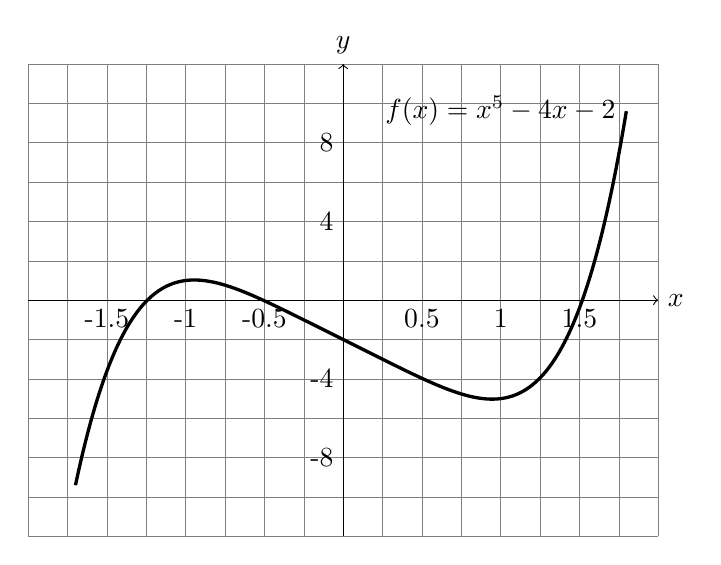
\begin{tikzpicture}[xscale=2, yscale=0.25, domain=-1.7:1.8, samples=200]
        % Draw grid lines
        \draw[very thin, color=gray] (-2,-12) grid [xstep=0.25, ystep=2] (2,12);
    
        % Add axes
        \draw[->] (-2,0) -- (2,0) node[right] {$x$};
        \draw[->] (0,-12) -- (0,12) node[above] {$y$};
    
        % Draw actual graph
        \draw[very thick, smooth, variable=\x] plot ({\x}, {\x^5 - 4*\x - 2}) node[left] {$f(x) = x^5 - 4x - 2$};
    
        % Add x-axis labels
        \node [below] at (-1.5,0) {-1.5};
        \node [below] at (-1,0) {-1};
        \node [below] at (-0.5,0) {-0.5};
        \node [below] at (0.5,0) {0.5};
        \node [below] at (1,0) {1};
        \node [below] at (1.5,0) {1.5};
    
        % Add y-axis labels
        \node [left] at (0,-8) {-8};
        \node [left] at (0,-4) {-4};
        \node [left] at (0,4) {4};
        \node [left] at (0,8) {8};
    \end{tikzpicture}
    \caption{Graph of $f(x) = x^5 - 4x - 2$}
\end{figure}

Do not be mislead by the graph of $f(x)$ -- one can easily verify that -1.25, 0.5, and 1.5 are \textit{not} zeroes of $f(x)$ in $\Q$.

\begin{proof}
    One sees by Eisenstein's Criterion (\myref{thrm-eisenstein-criterion}) with the prime 2 that $f(x)$ is irreducible over $\Q$; consequently this means that $f(x)$ is separable in $F$ (\myref{thrm-zeroes-of-an-irreducible}).

    We first argue that there are only 3 real zeroes for $f(x)$. We first produce a table of values of $f(x)$.
    \begin{table}[H]
        \centering
        \begin{tabular}{|l|l|}
            \hline
            $\boldsymbol{x}$ & $\boldsymbol{f(x)}$ \\ \hline
            -1.25 & $-\frac{53}{1024}$ \\ \hline
            -1 & 1 \\ \hline
            -0.75 & $\frac{781}{1024}$ \\ \hline
            -0.5 & $-\frac1{32}$ \\ \hline
            $\vdots$ & $\vdots$ \\ \hline
            1.5 & $-\frac{13}{32}$ \\ \hline
            1.75 & $\frac{7591}{1024}$ \\ \hline
        \end{tabular}
    \end{table}
    From this table, one sees that $f(x)$ changes sign from -1.25 to -1, from -0.75 to -0.5, and from 1.5 to 1.75. By the stated fact, this means that there are 3 distinct real zeroes from -1.25 to 1.75. Let these zeroes by denoted by $\alpha_1$, $\alpha_2$, and $\alpha_3$ respectively. Now, one sees for any $x < -1.25$ that
    \[
        4x + 2 > 4(-1.25) + 2 = -3 > (-1.25)^5 = -\frac{3125}{1024} > x^5
    \]
    which means that $x^5 - 4x - 2 < 0$ for all $x < -1.25$. Similarly,
    \[
        x^5 > 1.75^5 = \frac{16807}{1024} > 4(1.75) + 2 = 9 > 4x + 2
    \]
    for all $x > 1.75$, meaning $x^5 - 4x - 2 > 0$ for all $x > 1.75$. Therefore $\alpha_1$, $\alpha_2$, and $\alpha_3$ are the only 3 real zeroes of $f(x)$. Consequently the other two zeroes, which we call $\beta_1$ and $\beta_2$, are non-real and are present in $F$.

    Now, by the Factor Theorem (\myref{corollary-factor-theorem}), we may factor $f(x)$ as
    \[
        f(x) = (x-\alpha_1)(x-\alpha_2)(x-\alpha_3)(x^2 + Ax + B)
    \]
    for some $A, B \in \R$. On the other hand, knowing that $\beta_1$ and $\beta_2$ are the remaining two zeroes of $f(x)$ means that they must be the zeroes of $x^2 + Ax + B$. Using the quadratic formula we see that the zeroes of the quadratic are
    \[
        \frac{-A\pm\sqrt{A^2 - 4B}}{2} = -\frac{A}{2} \pm \frac{\sqrt{A^2-4B}}2
    \]
    and these must be the values of $\beta_1$ and $\beta_2$ (in some order). In particular we know that since $\beta_1$ and $\beta_2$ are non-real, thus $A^2 - 4B < 0$; consequently $\beta_1, \beta_2 \in \C$. In particular we may write $\beta_1 = a + bi$ and $\beta_2 = a-bi$ for some $a, b \in \R$. Hence we have found all 5 zeroes of $f(x)$, and so $F = \Q(\alpha_1, \alpha_2, \alpha_3, a+bi, a-bi)$.

    Now we proceed with determining the Galois group of $F/\Q$. \myref{prop-galois-field-automorphism-permutes-zeroes-of-polynomial} tells us that an element of $\Gal{F/\Q}$ permutes the zeroes of $f(x)$, and so Cayley's theorem (\myref{thrm-cayley}) tells us that $\Gal{F/\Q}$ is isomorphic to a subgroup of $\Sn{5}$ (since there are 5 zeroes), say $H$. Note also that
    \[
        [F:\Q] = [F:\Q(\alpha_1)][\Q(\alpha_1):\Q]
    \]
    by Tower Law (\myref{thrm-tower-law}) and $[\Q(\alpha_1):\Q] = 5$ as $\alpha_1$ is a zero of the degree 5 irreducible polynomial $f(x)$ over $\Q$. Hence $[F:\Q]$ is divisible by 5, and since $|\Gal{F/\Q}| = [F:\Q]$ by \myref{thrm-order-of-galois-group-is-degree-of-field-extension}, thus $|\Gal{F/\Q}|$ is also divisible by 5. So Cauchy's theorem (\myref{thrm-cauchy}) tells us that $\Gal{F/\Q}$ contains an element of order 5, meaning that $H$ contains a cycle of length 5. In addition, the automorphism
    \[
        \sigma: F \to F, u + vi \mapsto u - vi
    \]
    is an automorphism that fixes the real numbers and so fixes the rationals, meaning $\sigma \in \Gal{F/\Q}$. Note also that this automorphism fixes the 3 real zeroes ($\alpha_1$, $\alpha_2$, and $\alpha_3$) and interchanges the two complex zeroes ($a+bi$ and $a-bi$). Thus $\sigma^2 = \id$ and therefore $\sigma$ has order 2 in $\Gal{F/\Q}$, which means $H$ contains a 2-cycle (i.e., transposition). By \myref{lemma-subgroup-containing-transposition-and-maximal-length-cycle-is-whole-symmetric-group} we thus know that $H = \Sn{5}$ and so $\Gal{F/\Q} \cong \Sn{5}$.
\end{proof}

Why is it important that the Galois group of that polynomial is $\Sn{5}$? It turns out that $\Sn{5}$ is \textit{not} solvable.

\begin{proposition}
    $\Sn{5}$ is not a solvable group.
\end{proposition}
\begin{proof}
    We first find a composition series of $\Sn{5}$. Note that $\An{5}$ is a normal subgroup of $\Sn{5}$ (\myref{prop-An-normal-subgroup-of-Sn}), $|\Sn{5}| = 5! = 120$ (\myref{exercise-order-of-Sn}), and $|\An{5}| = \frac{5!}2 = 60$ (\myref{prop-order-of-An}). Since the order of a subgroup must divide the order of the group, the maximal order of a proper subgroup of $\Sn{5}$ is 60. Hence $\An{5}$ is the maximal (normal) subgroup of $\Sn{5}$. However $\An{5}$ is a simple group (\myref{thrm-An-is-simple-for-n>=5}) which means that it has no proper normal subgroups. Hence the composition series of $\Sn{5}$ is
    \[
        1 \lhd \An{5} \lhd \Sn{5}.
    \]
    
    However, note that the composition factor $\An{5}/1 \cong \An{5}$ is not a cyclic group of prime order. Therefore, by \myref{prop-solvable-equivalence-for-finite-groups}, we see that $\Sn{5}$ is not solvable.
\end{proof}

Therefore we see the following fact.

\begin{proposition}
    $x^5 - 4x - 2$ is not solvable by radicals over $\Q$.
\end{proposition}
\begin{proof}
    We know that the splitting field of $x^5 - 4x - 2$ over $\Q$, which we denote by $F$, has a Galois group isomorphic to $\Sn{5}$. But $\Sn{5}$ is not solvable. Hence, by the contrapositive of Galois' theorem (\myref{thrm-solvable-by-radicals-implies-solvable-group}), we see that the splitting field $F$ is not contained in a radical extension, which means that $f(x)$ is not solvable by radicals over $\Q$.
\end{proof}

The obvious generalisation of the above fact is captured by the Abel-Ruffini theorem.

\begin{theorem}[Abel-Ruffini]\index{Abel-Ruffini Theorem}\label{thrm-abel-ruffini}
    A general polynomial with real coefficients with degree of 5 or more is not solvable by radicals.
\end{theorem}
\begin{proof}
    See \myref{exercise-prove-abel-ruffini} (later).
\end{proof}

\begin{exercise}\label{exercise-prove-abel-ruffini}
    Prove \myref{thrm-abel-ruffini}.
\end{exercise}

\newpage

\section{Problems}
% TODO: Add

% \begin{problem}
%     Let $\theta \in \R$. \textbf{De Moivre's formula}\index{De Moivre's formula} states that
%     \[
%         (\cos\theta + i\sin\theta)^n = \cos(n\theta) + i\sin(n\theta)
%     \]
%     for all non-negative integers $n$.
%     \begin{partquestions}{\roman*}
%         \item Prove De Moivre's formula.
%         \item Deduce a primitive $n$th root of unity in $\C$, proving your answer.
%     \end{partquestions}
% \end{problem}

% \begin{problem}
%     Prove that $\Sn{n}$ is \textit{not} solvable for all $n \geq 5$.
% \end{problem}
